\documentclass[11pt, oneside]{article}   	% use "amsart" instead of "article" for AMSLaTeX format
\usepackage{geometry}                		% See geometry.pdf to learn the layout options. There are lots.
\geometry{letterpaper}                   		% ... or a4paper or a5paper or ... 
%\geometry{landscape}                		% Activate for rotated page geometry
%\usepackage[parfill]{parskip}    		% Activate to begin paragraphs with an empty line rather than an indent
\usepackage{graphicx}				% Use pdf, png, jpg, or eps§ with pdflatex; use eps in DVI mode
								% TeX will automatically convert eps --> pdf in pdflatex		
\usepackage{amssymb}

\usepackage{indentfirst}

\usepackage{amsmath}

\newcommand\tab[1][1cm]{\hspace*{#1}}				% Define tab command and spacing
\renewcommand{\baselinestretch}{1.5}				% Define the line spacing
\newcommand{\rpm}{\raisebox{.2ex}{$\scriptstyle\pm$}}	% Define +/- for math script
\newcommand*\mean[1]{\overline{#1}}				% Define the bar over symbol to indicate mean

\graphicspath{ {./figures/} }

\title{NE255 Final Report: \\
Deterministic solution of TE in 1-D spherical coordinates}
\author{Milos Atz}
\date{December 13, 2016}							

% math syntax for NTE Equation (from R. Slaybaugh NE155 tex notes)
\newcommand{\nth}{n\ensuremath{^{\text{th}}} }
\newcommand{\ve}[1]{\ensuremath{\mathbf{#1}}}
\newcommand{\Macro}{\ensuremath{\Sigma}}
\newcommand{\rvec}{\ensuremath{\vec{r}}}
\newcommand{\omvec}{\ensuremath{\hat{\Omega}}}
\newcommand{\vOmega}{\ensuremath{\hat{\Omega}}}

\begin{document}

\maketitle

\section{Introduction}

For a geologic repository containing fissile materials, a criticality safety assessment (CSA) is necessary to ensure subcriticality. The CSA should cover (1) the canister environment, (2) the near field, which includes the engineered barriers, and (3) the far field, where fissile material from multiple canisters can accumulate in geologic formations after canister failure and subsurface transport \cite{ahn1}. The far-field case is complicated by long timescales and uncertainties regarding material compositions and geometry. One way to assess the far-field criticality risk is by using conservative neutronic analysis alongside deterministic transport models \cite{ahn1}. Understanding how the multiplication factor and critical mass of a deposition of fissile material behave under variable conditions can allow insights into mitigating criticality risk by controlling fuel cycle management, waste processing, and repository design.

In previous work, criticality calculations have been carried out using MCNP v.6.1 \cite{xudong} \cite{mcnp}. While MCNP can produce good estimates of the multiplication factor, the calculations are expensive when performing parametric study and iterating to find the minimum critical mass. A deterministic model can give results more quickly than MCNP. At the very least, such a model can be used to validate findings in MCNP. If expanded with an extensive data library, it could grow into more. In this work, a 1-D discrete ordinates transport solver for a two-region spherical geometry in curvilinear coordinates is developed. Applied to criticality safety, the model represents a water-saturated deposition of fissile material in host rock with a reflector of the host rock material.

% with an option to solve for a criticality eigenvalue.
\section{Mathematics}

Using curvilinear coordinates in the discrete ordinates method allows for straightforward treatment of spherical systems. The geometry can be considered 1-D. In 1-D curvilinear coordinates, the angular flux, $\psi(\rho, \mu)$ is dependent on only $\rho$, the distance from the origin, and $\mu$, the directional cosine of $\hat{\Omega}$ with respect to the radial direction at $\rho$. The transport equation in spherical coordinate is shown below \cite{lm}.
%
\begin{equation}\label{eq:spherical_te}
	\mu\frac{\partial}{\partial\rho}\psi(\rho, \mu)+
	\frac{(1-\mu^2)}{\rho}\frac{\partial}{\partial\mu}\psi(\rho, \mu)+
	\sigma(\rho)\psi(\rho, \mu) = 
	q(\rho, \mu)
\end{equation}
%
In Equation \ref{eq:spherical_te}, the first two terms represent streaming with respect to position and angle. The second term is the total interaction term, where $\sigma$ is the total cross section. On the right hand side, $q$ is this emission density \cite{lm}:
%
\begin{equation}\label{eq:emission_density}
q(\rho, \mu) = \sum_{l=0}^{L}(2l+1)\sigma_l(\rho)P_l(\mu)\phi_l(\rho)+s(\rho, \mu)
\end{equation}
%
In Equation \ref{eq:emission_density}, the $\phi_l$ are the Legendre moments of the angular flux. To ensure that any approximations to the transport equation retains its particle conservation properties, it is often written in conservation form, which requires rewriting the streaming operator \cite{lm}:
%
\begin{equation}\label{eq:conservation_te}
	\frac{\mu}{\rho^2}\frac{\partial}{\partial\rho}\rho^2\psi(\rho, \mu)+
	\frac{1}{\rho}\frac{\partial}{\partial\mu}(1-\mu^2)\psi(\rho, \mu)+
	\sigma(\rho)\psi(\rho, \mu) = 
	q(\rho, \mu)
\end{equation}
%

In discrete ordinates, angle and space must be discretized, and curvilinear coordinates is no exception. However, the discretization is different than for Cartesian coordinates. As a particle streams through the system, its position and its angle change relative to the reference point (the origin of the sphere). Thus, two layers of discretization are necessary and the equations must be treated in a special way. In Appendix A, the discretization in angle and space are derived in full; derivations are sourced entirely  based on from the "Computational Methods of Neutron Transport" by E. E. Lewis and W. F. Miller \cite{lm}. 

A radial mesh is imposed on the sphere dividing it into concentric cells with centers at positions $\rho_i$. The inner and outer bounds of the cells are $\rho_{i-1/2}$ and $\rho_{i+1/2}$ respectively. The cell average flux is defined as follows, where $V_i$ is the volume of the cell.
%
\begin{equation}
\psi_{ni} = \frac{1}{V_i}4\pi\int_{\rho_{i-1/2}}^{\rho_{i+1/2}}{d\rho\rho^2\psi_n(\rho)}
\end{equation}
%
Angle is discretized by expanding the angular flux in the first $N+1$ Legendre polynomials $P_N$. Gaussian quadrature is used so that each $\mu_n$ in the set of $N$ $\mu$ are taken to be the roots of $P_N(\mu_n) = 0, n=1, 2,...,N$, where $P_N$ is . The quadrature weights are determined such that the quadrature correctly integrates the Legendre polynomials $P_0(\mu)$ through $P_{N-1}(\mu)$.
%
\begin{equation}
\frac{1}{2}\sum_{n=1}^N{w_n P_l(\mu_n)} = \delta_{l0}, \tab l = 0, 1, ..., N-1
\end{equation}
%
The treatment of angle in curvilinear coordinates is tricky. Angular differencing coefficients $\alpha_{n\pm1/2}$ are required to difference in angle while continuing to use commonly used quadratures like Gaussian quadrature. These coefficients are appear in the equation used to solve for cell average flux in each cell. 
%
\begin{equation}\label{eq:spatialdd}
\begin{aligned}
\psi_{ni} = \left[ 2\left| \mu_n \right| A_{i \mp 1/2} + \frac{4}{w_n}\left(A_{i+1/2}-A_{i-1/2}\right)\alpha_{n+1/2}+V_i\sigma_i \right]^{-1} \\
\times \bigg( \left| \mu_n \right| \left(A_{i+1/2}-A_{i-1/2}\right)\psi_{n,i \pm 1/2} + \\
\frac{2}{w_n}\left(A_{i+1/2}-A_{i-1/2}\right)\left(\alpha_{n+1/2}-\alpha_{n-1/2}\right)\psi_{n-1/2,i}+V_i Q_{ni} \bigg), \\
\mu \lessgtr 0
\end{aligned}
\end{equation}
%
There are three terms in Equation \ref{eq:spatialdd}, each divided by the same denominator (the first line). The first term represents particles incoming from the preceding cell in space $i \pm 1/2$ into the current cell $i$. The second term represents particles incoming from the previous half-angle $n-1/2$ into the current angle $n$. The third term is particles that are born in cell $i$. The denominator accounts for particles leaving the cell and particles that are absorbed in the cell. This equation, solved alongside the diamond difference relationships in space and angle in Equations \ref{eq:dd_angle} and \ref{eq:dd_space}, is used to solve for the flux in the sphere.
%
\begin{equation}\label{eq:dd_angle}
\psi_{n+1/2,i} = 2\psi_{n,i}-\psi_{n-1/2,i}
\end{equation}
%
\begin{equation}\label{eq:dd_space}
\psi_{n,i \pm 1/2} = 2\psi_{n,i}-\psi_{n,i\mp1/2}
\end{equation}

\section{Algorithms}

The space-angle sweep in curvilinear coordinates is similar to that in Cartesian coordinates. In spherical geometry, the starting angle is radially inward, $\mu = -1$ and starting spatial mesh cell is the outermost cell. Starting with $\psi_{1/2, I+1/2}$, the march proceeds inward (decreasing $i$), sequentially solving for each $\psi_{1/2, i}$ using Equation \ref{eq:starting_flux}. 
%
\begin{equation}\label{eq:starting_flux}
\psi_{1/2, i} = \frac{2\psi_{1/2, i+1/2}+\left(\rho_{i+1/2} - \rho_{i-1/2}\right)Q_{ni}}{2+\sigma_i\left(\rho_{i+1/2} - \rho_{i-1/2}\right)}
\end{equation}
%
Then, the $\psi_{1,i}$ are calculated, again starting from the outermost cell. This goes on until all angular fluxes for $\mu_n<0$, ($n \leq N/2$) are known. Then, the starting fluxes at $i=1/2$ for $n > N/2$ are determined and the process is repeated, except this time with $\mu > 0$. These fluxes are combined according to the quadrature with the fluxes from the inward sweep and are used to update the scattering source for the next iteration. Figure \ref{fig:algorithm} demonstrates the process graphically for $N=4$ \cite{lm}.
%
\begin{figure}\label{fig:algorithm}
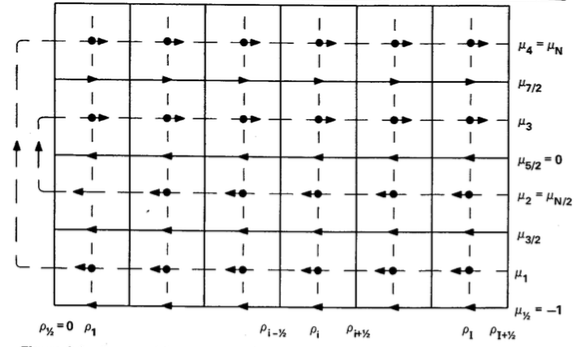
\includegraphics[width=14cm]{algorithm}
\caption{Space-angle mesh sweep for 1-D spherical geometry \cite{lm}.}
\end{figure}

\section{Code Use}

Using the code requires the user to have Python and numerous packages, all available and automatically installed with Anaconda. The code is written in a detailed and commented Jupyter notebook so that the user can see inside the algorithm and implementation. Compilation of the code has been started but not completed because the code isn't yet fully functional (teaser, more details to come). Readers are encouraged to view the notebook to understand the details and subroutines.

Currently, the user supplies many inputs that specify various aspects of the problem.
%
\begin{itemize}
\item Radius of the core
\item Number of cells in the core
\item Degree of Gaussian quadrature ($N$)
\item Order of $P_N$ expansion of scattering ($L$)
\item The incoming flux at the sphere edge
\item $\Sigma_{tot}, \Sigma_{s}$
\end{itemize}
%
The user also specifies the type of source, either a point source or a uniform source. If a point source is selected, the user must identify where the point source is located. If the user desires a reflecting region around the core, they must also specify the following for the reflector:
%
\begin{itemize}
\item Thickness of the reflector
\item Number of cells in the reflector
\item $\Sigma_{tot}, \Sigma_{s}$
\end{itemize}
%

\section{Test Problems and Results}

In this section, we will come to the unfortunate realization that the code doesn't work and will discuss some reasons for why that might be. To try and simplify that discussion, the reflector is omitted in all tests, so the results presented here are for a bare spherical system. Three test problems are identified to check the performance of the code without a reflector. All are easy to solve either conceptually or with diffusion theory. These solutions are implemented in code in an accompanying Jupyter notebook.

\begin{enumerate}
\item Bare sphere, uniform, isotropic source in near-infinite medium, no scattering
\item Bare sphere, isotropic point source at the center of the sphere
\item Bare sphere, uniform external source
\item Two region bare sphere, inner region has uniform external source 
\end{enumerate}

The solution to the near-infinite system with uniform, isotropic source is a constant with respect to position and angle: $\phi = S/\sigma$. If the system is large enough, this result should be obtainable by the code. This is also the case used by Lewis and Miller \cite{lm} to refine the angular differencing in the derivation of the discretization. Figure \ref{fig:near_inf_uniform} shows the flux as a function of radius in the sphere with isotropic external source $s_o = 40.0$ and total cross section $\sigma = 4.0$. For this figure, Gaussian quadrature of degree $N=4$ is used.
%
\begin{figure}
\centering
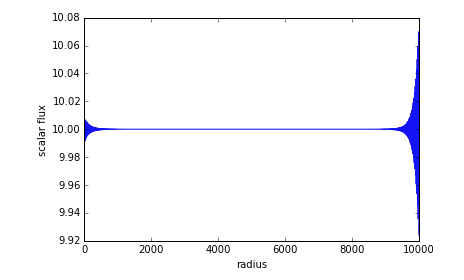
\includegraphics[width=11cm]{uniform_src_near_inf}
\caption{Solution for flux in a bare sphere with uniform isotropic source with no scattering. In this system the flux equals the source (40.0) divided by the cross section (4.0).}
\label{fig:near_inf_uniform}
\end{figure}
%
The result shows flux constant across space with the exception of oscillations that arise near the origin and by the boundary. These are the focus of later discussions because the quality of the result suffers near the origin and by the boundary, in some problems to the point that the answer is clearly wrong. More on that later.

The second test problem involves introducing scattering. The diffusion solution to this equation is straightforward and is shown in Equation \ref{eq:pt_src_diff}.
%
\begin{equation}\label{eq:pt_src_diff}
\phi(r) = \frac{s_o\sinh((R-r)/L)}{4\pi D \sinh(R/L)}
\end{equation}
%
In the transport solution, scattering is expanded in Legendre polynomials according to the $P_N$ method with order $L=4$. A source is placed in the first cell. In the result, plotted in Figure \ref{fig:origin_pt_source}, the degree of Gaussian quadrature is $N=2$ and 20 radial mesh cells of uniform width are used. The diffusion result is plotted in the same figure, according to the equation for flux. Both the diffusion and code solutions used source values of $s_o = 10.0$, $\sigma_{tot} = 4.0$, $\sigma_s = 2.0$.
%
\begin{figure}
\centering
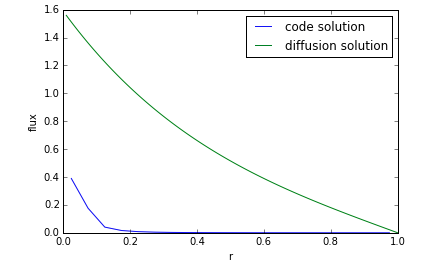
\includegraphics[width=11cm]{origin_pt_source_soln}
\caption{Comparison of diffusion and code solutions for point source at center of sphere.}
\label{fig:origin_pt_source}
\end{figure}
%
This is an unfortunate result. Though the code solution appears to behave somewhat properly, the magnitude of the difference between the two solutions is high. If the diffusion solution is taken to be ``more correct'', it would seem as though the code is underpredicting the scattering contribution to the flux.

Things get worse when assessing the third test problem, a bare sphere with uniform distributed source with scattering. The solution by the diffusion approximation is given by Equation \ref{eq:dist_src_diff} \cite{lewis_fundamentals}.
%
\begin{equation}\label{eq:dist_src_diff}
\phi(r) = \frac{-s_o(R+a)}{\Sigma_a \sinh((R+a)/L)}\frac{1}{r}\sinh(r/L)+\frac{s_o}{\Sigma_a}
\end{equation}
%
\begin{figure}
\centering
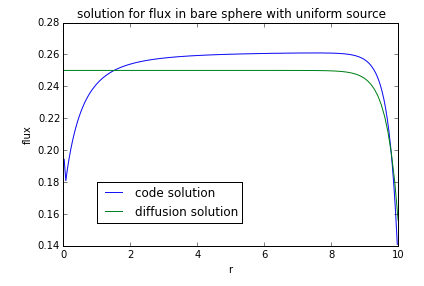
\includegraphics[width=11cm]{uniform_src}
\caption{Comparison of the code and diffusion solutions for flux in a bare sphere with uniform source.}
\label{fig:uniform_src_comp}
\end{figure}
%
The solution is obtained from the code using 200 uniformly distributed radial meshes, Gaussian quadrature of degree $N=2$ and scattering expansion with $L=4$. The source in both diffusion and code solutions is $s_o=0.5$ and cross sections are $\sigma_{tot} = 2.5$, $\sigma_s = 0.5$. Ignoring the behavior at the origin, the code performs reasonably well compared to the diffusion solution. 

The behavior at the origin is difficult to assess, but we can get better insight into the behavior of the code by examining the angular flux and half-angle fluxes at convergence. Figure  \ref{fig:detailed_flux_break_down} shows the same code solution but includes the angular and half-angle fluxes in the $\pm \mu$ directions. Because $N=2$, the blue dots mark the "starting flux", when $n=1/2$. Based on this half-angle flux, the angular flux represented by the blue line is calculated for $n=1$. Similarly, the red dots mark the half-angle flux where $n=3/2$ and the red line is the angular flux for $n=2$. The green line is the scalar flux. The sharp dip in angular flux for $n=2$ at the origin is due to the difference between the incoming flux at the origin, which converges to 0.2537 in this example, and the low half-angle flux (red dots).
%
\begin{figure}
\centering
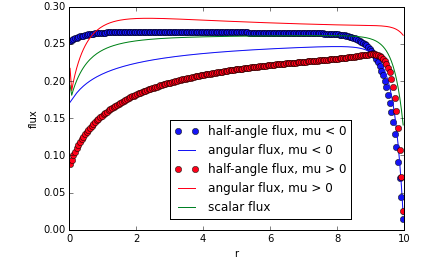
\includegraphics[width=11cm]{uniform_src_detailed}
\caption{Breakdown of the half angle and angular fluxes that comprise the code solution for uniform source in bare sphere.}
\label{fig:detailed_flux_break_down}
\end{figure}

At this time, these issues have not been fully diagnosed. The fluxes behave appropriately at the boundary and give reasonable results through the majority of the sphere. I suspect that there are issues with the treatment of flux at the center and the integration of the angular fluxes. However, despite many frustrating hours, I have not been able to find these issues in my algorithm.

Finally, the fourth test problem demonstrates the use of the reflector. The diffusion solution for a two region bare sphere in which the inner sphere has a uniform source is given by Equations \ref{eq:two_reg_diff_sph1} and \ref{eq:two_reg_diff_sph2}. The constants are given in \ref{eq:two_reg_constants1} and \ref{eq:two_reg_constants2}; $A$, $B$, $C$, and $D$ are constants whose values can be found along with the full derivation in a supplemental Jupyter notebook \cite{lewis_fundamentals}.
%
\begin{equation}
\begin{aligned}
\phi(r) = \frac{2C_1}{r}\sinh(r/L)+\frac{s_o}{\Sigma_{a,1}}, \tab 0 \le r < R_{1}
\end{aligned}
\label{eq:two_reg_diff_sph1}
\end{equation}
%
\begin{equation}
\phi(r) = \frac{C_3}{r}e^{\frac{r}{L_2}}
-\frac{C_3}{r}e^{2\frac{R_2+a}{L_2}}e^{\frac{-r}{L_2}}, \tab R_1 \le r < R_2
\label{eq:two_reg_diff_sph2}
\end{equation}
%
\begin{equation}
C_1 =\left(\frac{C_3}{R_1}\left[e^{\frac{R_1}{L_2}}-Ae^{-\frac{R_1}{L_2}}\right] - \frac{s_o}{\Sigma_{a,1}}\right)
\label{eq:two_reg_constants1}
\end{equation}
%
\begin{equation}
C_3 = \frac{2 D_1 s_o}{\Sigma_{a,1}}
\left[\frac{2 D_1}{R_1}\left(e^{\frac{R_1}{L_2}}
-Ae^{-\frac{R_1}{L_2}}\right)-\frac{DB}{C} \right]^{-1}
\label{eq:two_reg_constants2}
\end{equation}

The diffusion solution and the code solution are plotted in Figure \ref{fig:refl_soln} for the case where the radius of the core and reflector thickness are $R_1 = 5.0$ and $R_t = 10.0$, respectively. The total and scattering cross sections are set to 2.0 and 1.0, respectively, in the core, and 5.0 and 2.0, respectively, in the reflector. The uniform flux in the core is $s_o$ = 0.8. The code solution used quadrature degree $N=2$ and scattering expansion order $L=4$.
%
\begin{figure}
\centering
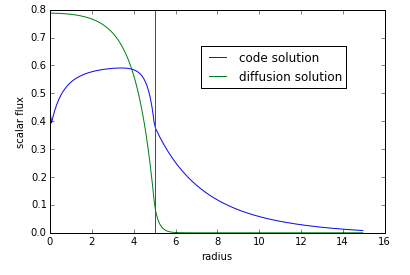
\includegraphics[width=11cm]{reflector_result}
\caption{Comparison of code output with diffusion result for two region sphere; the red line marks the interface between the two regions}.
\label{fig:refl_soln}
\end{figure}

The code results matches up somewhat reasonably with the diffusion result, again with the exception of the behavior at the origin.

\section{Summary}

In this work, we covered the implementation of a solver for the neutron transport equation in 1-D spherical coordinates in a variety of settings: with uniform and point sources, bare and reflected. The derivation and explanations of the special treatment required to handle the change in reference position and angle as the particle streams are discussed (in detail in Appendix A). The code result is shown to produce reasonable results for simple problems but shows erratic behavior at the origin, as evidenced when comparing it against diffusion approximation results for similar systems. More work is required to diagnose and address this issue. Future work can and should involve compiling and packaging the code into a nice, user-friendly product.

\begin{thebibliography}{1}

  \bibitem{ahn1} Joonhong Ahn. {\em Criticality Safety of Geologic Disposal for High-Level Radioactive Wastes} 2006: Nuclear Engineering and Technology v38:6.

  \bibitem{xudong} Xudong Liu, Joonhong Ahn, Fumio Hirano. {\em Conditions for criticality by uranium deposition in water-saturated geological formations} 2014: Journal of Nuclear Science and Technology v.52
   
   \bibitem{mcnp} D.B. Pelowitz, ed. {\em MCNP6TM User?s Manual} 2011, Los Alamos.
   
   \bibitem{lm} E.E. Lewis and W.F. Miller. {\em Computational Methods of Neutron Transport} 1984: John Wiley \& Sons.
   
   \bibitem{lewis_fundamentals} E.E. Lewis. {\em Fundamentals of Nuclear Reactor Physics} 2008: Academic Press.
   
\end{thebibliography}

\appendix

\section{Discretization of the TE in 1-D spherical coordinates}

\subsection{Angular Discretization}

In curvilinear coordinates, we can attempt to represent angle as a set of discrete ordinates equations, analogous to the treatment in slab geometry. We evaluate the equation at the same $\mu_n$ as in the slab geometry. However, because of the different nature of the curvilinear equations, this procedure can no longer be considered as tracing neutrons along discrete paths through space. If we want to utilize desirable quadrature sets (e.g. Gauss and double Gauss quadrature), the angular redistribution effects caused by curvilinear coordinates must be taken into account. Suppose, for example, a diamond differencing relationship like the one in Equation \ref{eq:angular_approx} is applied directly to Equation \ref{eq:conservation_te}.
%
\begin{equation}\label{eq:angular_approx}
\psi(\rho, \mu_n) \approx \frac{1}{2}\left[\psi(\rho, \mu_{n+1/2})+\psi(\rho, \mu_{n-1/2})\right]
\end{equation}
%
This simple method places too many restrictions on the ordinates for even simple problems. The solution to Equation \ref{eq:conservation_te} for a uniform isotropic source in an infinite medium is just a constant, $\psi = S/\sigma$. In that case, the sum of the two streaming terms in Equation \ref{eq:conservation_te} sould vanish. For this to be true, $\psi(\rho, \mu_{n\pm1/2})=\psi(\rho, \mu_n)=\phi$. Using the approximation in Equation\ref{eq:angular_approx} requires $\mu_n$ to be the average of $\mu_{n+1/2}$ and $\mu_{n-1/2}$. Gauss and double Gauss quadrature do not meet this constraint even when $N=2$. Instead, angular differencing coefficients are introduced into the conservation form of the transport equation in spherical geometry in Equation \ref{eq:conservation_te}. Here, $n$ represents an angle from the quadrature set, and $\psi_n(\rho) = \psi(\rho, \mu_n)$ for $\mu_1 < \mu_2 < \dots < \mu_N$ with $\mu_{1/2} \equiv -1$ and $\mu_{N+1/2} = 1$.
%
\begin{equation}\label{eq:conservation_te_angular_difference}
\frac{\mu_n}{\rho^2}\frac{\partial}{\partial\rho}\rho^2\psi_n(\rho)+
\frac{2}{\rho w_n}\left[\alpha_{n+1/2}\psi_{n+1/2}(\rho)-\alpha_{n-1/2}\psi_{n-1/2}(\rho)\right]+
\sigma(\rho)\psi_n(\rho) = 
q_n(\rho)
\end{equation}
%
This method can account for the disappearance of the streaming term required to correctly solve for a uniform isotropic flux in an infinite medium. In order to ensure this result, each $\alpha_{n+1/2}$ is defined recursively. If the value of $\alpha_{1/2}$ is known, all  $\alpha_{n+1/2}$ can be determined uniquely in terms of quadrature parameters.
%
\begin{equation}\label{eq:recursive_alpha}
\alpha_{n+1/2} = \alpha_{n-1/2}-\mu_n w_n
\end{equation}
%
In addition, Equation \ref{eq:conservation_te_angular_difference} must obey the neutron balance condition, which is obtained by integrating Equation \ref{eq:conservation_te}, where $\phi$ is the scalar flux, $S$ is the source, $J$ is the current, and $\sigma_r = \sigma - \sigma_0$.
%
\begin{equation}\label{eq:nbal_raw}
\frac{1}{\rho^2}\frac{\partial}{\partial\rho}\rho^2J(\rho)+
\sigma_r(\rho)\phi(\rho)=
S(\rho)
\end{equation}
%
Expressed in terms of the discrete ordinates, Equation \ref{eq:nbal_raw} becomes the following:
%
\begin{equation}\label{eq:nbal_disc}
\frac{1}{\rho^2}\frac{\partial}{\partial\rho}\rho^2\frac{1}{2}\sum_{n=1}^N{w_n\mu_n\psi_n(\rho)}+
\sigma_r(\rho)\frac{1}{2}\sum_{n=1}^N{w_n\psi_n(\rho)}=
S(\rho)
\end{equation}
%
Equation \ref{eq:conservation_te_angular_difference} meets this condition when weighted by $w_n$ and summed of $n$ if:
\newline
\begin{equation}\label{eq:alpha_nbal_condition}
\sum_{n=1}^N\left[\alpha_{n+1/2}\psi_{n+1/2}(\rho)-\alpha_{n-1/2}\psi_{n-1/2}(\rho)\right]=\\
\alpha_{1/2}\psi_{1/2}(\rho)-\alpha_{N+1/2}\psi_{N+1/2}(\rho)=0
\end{equation}
%
Any quadrature set that is even in $\mu$ will produce $\alpha_{N+1/2}=0$ if $\alpha_{1/2}=0$, thus satisfying the condition. With these equations, we can create a set of coupled equations using diamond differencing in angle. Solving $\psi_n(\rho)=\frac{1}{2}\left[\psi_{n+1/2}(\rho)+\psi_{n-1/2}(\rho)\right]$ for $\psi_{n+1/2}$ and substituting into equation \ref{eq:conservation_te_angular_difference} gives the following:
%
\begin{equation}\label{eq:ddte}
\begin{aligned}
\frac{\mu_n}{\rho^2}\frac{\partial}{\partial\rho}\rho^2\psi_n(\rho)+
\frac{2}{\rho w_n}\left[2\alpha_{n+1/2}\psi_{n}(\rho)-(\alpha_{n+1/2}+\alpha_{n-1/2})\psi_{n-1/2}(\rho)\right]+\\
\sigma(\rho)\psi_n(\rho) =
q_n(\rho)
\end{aligned}
\end{equation}
%
The diamond difference relationship and Equation \ref{eq:ddte} together can be solved successively for $\psi_1, \psi_{3/2}, \psi_2, \dots, \psi_N$. To find $\psi_{1/2}$, $\mu_{1/2}=1$ is defined as the radially inward direction.

\subsection{Spatial Discretization}

As in Cartesian spatial differencing, finite volume method is used to discretize space. Equation \ref{eq:ddte} is first integrated over incremental volume $V_i$ with spherical shell surface area $A_i$ and a differencing relationship is applied. The radial mesh is defined in terms of $\rho$ and cross sections are assumed constant in each region. The cell averaged flux and source are defined as follows:
%
\begin{equation}\label{cell_avg_flux_A}
\psi_{ni} = \frac{1}{V_i}4\pi\int_{\rho_{i-1/2}}^{\rho_{i+1/2}}{d\rho\rho^2\psi_n(\rho)}
\end{equation}
%
\begin{equation}\label{cell_avg_source}
Q_{ni} = \frac{1}{V_i}4\pi\int_{\rho_{i-1/2}}^{\rho_{i+1/2}}{d\rho\rho^2 q_n(\rho)}
\end{equation}
%
We also make the approximation
%
\begin{equation}\label{flux_over_area}
4\pi\int_{\rho_{i-1/2}}^{\rho_{i+1/2}}{d\rho\rho\psi_n(\rho)} = \left(A_{i+1/2}-A_{i-1/2}\right)\psi_{ni}
\end{equation}
%
The spatial mesh is applied to Equation \ref{eq:ddte}. Integrating over $V_i$, applying the above cell-average approximations, and dividing by $V_i$ yields the equations required to sweep through the spatial mesh. For $\mu \lessgtr 0$.
%
\begin{equation}
\psi_{n,i \mp 1/2}=2\psi_{ni} - \psi_{n,i \pm 1/2} 
\end{equation}
%
\begin{equation}\label{eq:spatialdd_A}
\psi_{ni} = \frac{\left| \mu_n \right| \left(A_{i+1/2}-A_{i-1/2}\right)\psi_{n,i \pm 1/2}+
\frac{2}{w_n}\left(A_{i+1/2}-A_{i-1/2}\right)\left(\alpha_{n+1/2}-\alpha_{n-1/2}\right)\psi_{n-1/2,i}+V_i Q_{ni}}
{2\left| \mu_n \right| A_{i \mp 1/2} + \frac{4}{w_n}\left(A_{i+1/2}-A_{i-1/2}\right)\alpha_{n+1/2}+V_i\sigma_i}
\end{equation}
%
The starting direction is approximated by the following, which is solved for $\psi_{1/2,i}$ and plugged into Equation \ref{eq:spatialdd_A}.
%
\begin{equation}
-\frac{\left(\psi_{1/2, i+1/2} - \psi_{1/2, i-1/2}\right)}{\rho_{i+1/2}-\rho_{i-1/2}}+\sigma_i\psi_{1/2,i}=Q_{ni}
\end{equation}
%
The symmetry at the center of the sphere (in this case, the origin) is most often approximated by $\psi_{N+1-n, 1/2} = \psi_{n,1/2}$ for $n=1, 2, \dots, N/2$. However, due to truncation error, a small nonphysical dip in spatial flux can occur at the origin. To improve accuracy numerically, the condition that is actually implemented is $\psi_{n-1/2, 1/2} = \psi_{n+1/2, 1/2}$ for $n=1, 2, \dots, N$. The starting direction calculation determines $\psi_{1/2, 1/2}$ at the origin.

\end{document}
